\documentclass[12pt]{article}
\usepackage[margin=1in]{geometry}
\usepackage{graphicx}
\usepackage{booktabs}
\usepackage{amsmath}
\usepackage[hidelinks,draft]{hyperref}
\usepackage{natbib}
\usepackage{setspace}
\usepackage{float}
\usepackage{caption}
\usepackage{subcaption}
\usepackage{xcolor}

\singlespacing
\setlength{\parskip}{0.5em}
\setlength{\parindent}{0em}

\title{\textbf{Report 1: Are Headtracking Measures an Indicator of Depressive Symptoms?}\\[0.5em]
\large Preliminary Data Visualization, Descriptive Statistics, and Inferential Analysis}
\author{Parv Shah (2025201093) \and Hardik (2025201046) \and Gaurav (2025201065)}
\date{February 2026}

\begin{document}
\maketitle

% ──────────────────────────────────────────────────────────────────────────────
\section{Introduction}
% ──────────────────────────────────────────────────────────────────────────────

Depression is a leading cause of disability worldwide, yet objective behavioral markers remain limited. While self-report instruments such as the Patient Health Questionnaire (PHQ-9; \citealt{kroenke2001phq9}) are widely used for screening, they are inherently subjective. An emerging line of research investigates \textit{psychomotor retardation}---the slowing of physical movement and thought---as an observable correlate of depression \citep{bennabi2013psychomotor}. The anhedonia component of depression, in particular, may manifest as reduced exploratory behavior when individuals are placed in stimulating environments.

Recent work by \citet{srivastava2025headscan} demonstrated that headtracking data collected during 360° virtual reality (VR) video viewing could distinguish individuals based on depression severity. Using ANCOVA to control for anxiety (GAD-7 and STAI-T), they found that \textit{scanning speed}---the rate of angular head movement across the visual field---was significantly lower in the moderate-severe depression group compared to mild and minimal groups ($p < .001$, $\eta^2 = .295$, Cohen's $d = 1.64$). The present study is a \textbf{replication} of this work, conducted with college students in India using a Meta Quest 3 VR headset.

Participants viewed five 360° videos spanning different emotional contexts (abandoned buildings, a beach, a campus, a horror scene, and surfing) and completed standardized measures of depression (PHQ-9), anxiety (GAD-7; \citealt{spitzer2006gad7}; STAI-T; \citealt{spielberger1983stai}), current mood (PANAS-SF; \citealt{watson1988panas}), presence, and simulator sickness (VRNQ-VRISE; \citealt{kourtesis2019vrnq}).

Since depression and anxiety are highly covariant constructs \citep{kalin2020anxiety}, any analysis of depression-related differences must account for this overlap. This report presents preliminary descriptive statistics, visualizations, and initial inferential tests to characterize the dataset and set the stage for more advanced analyses in Report~2.

% ──────────────────────────────────────────────────────────────────────────────
\section{Methods}
% ──────────────────────────────────────────────────────────────────────────────

\subsection{Participants}
Forty college students (36 male, 4 female; age $M = 22.8$, $SD = 1.8$, range 19--27) participated. Sixteen (40\%) reported prior VR experience. Participants were recruited via convenience sampling.

\subsection{Materials}
Five 360° videos were used:
\begin{itemize}
    \item \textbf{V1}: Abandoned Buildings (60s) --- eerie, low valence
    \item \textbf{V2}: Evening at the Beach (60s) --- pleasant, calm
    \item \textbf{V3}: Campus (60s) --- neutral, familiar
    \item \textbf{V4}: The Nun Horror ($\approx$3 min) --- high arousal, negative
    \item \textbf{V5}: Tahiti Surf ($\approx$3 min) --- high arousal, positive
\end{itemize}
Videos were viewed on a Meta Quest 3 headset. Surveys were administered via PsyToolKit.

\subsection{Measures}
\begin{enumerate}
    \item \textbf{Headtracking}: Pitch (X), Yaw (Y), and Roll (Z) rotation changes and speeds recorded at $\approx$70 Hz. Summary measures computed per participant per video: mean rotation speed (total and per axis), standard deviation, median speed, mean absolute rotation change, range of angular exploration, and peak speed.
    \item \textbf{PHQ-9}: 9-item depression screener (0--27). Clinical cutoff of $\geq 10$ used for moderate depression \citep{kroenke2001phq9}.
    \item \textbf{GAD-7}: 7-item generalized anxiety measure (0--21) \citep{spitzer2006gad7}.
    \item \textbf{STAI-T}: 20-item trait anxiety inventory (20--80) \citep{spielberger1983stai}.
    \item \textbf{PANAS-SF}: 20-item affect schedule measuring positive and negative affect pre- and post-VR \citep{watson1988panas}.
    \item \textbf{VRNQ-VRISE}: 5-item simulator sickness subscale (5--35) \citep{kourtesis2019vrnq}.
    \item \textbf{Emotion ratings}: Valence (1--9, unpleasant--pleasant) and Arousal (1--9, calm--excited) per video.
    \item \textbf{Presence}: 5-item immersion measure (5--35) per video.
\end{enumerate}

\subsection{Depression Group Classification}
Participants were classified as \textit{Depressed} (PHQ-9 $\geq 10$; $n = 8$) or \textit{Non-Depressed} (PHQ-9 $< 10$; $n = 32$) using the established clinical cutoff for moderate depression \citep{kroenke2001phq9}. The original study by \citet{srivastava2025headscan} used three depression groups (minimal, mild, moderate-severe) with $\geq 10$ marking the moderate-severe threshold; we adopt the same cutoff for a binary split given our smaller sample.

\subsection{Statistical Approach}
\begin{itemize}
    \item \textbf{Descriptive statistics}: Means, standard deviations, medians, and ranges for all key variables.
    \item \textbf{Normality testing}: Shapiro-Wilk tests to assess distributional assumptions.
    \item \textbf{Correlations}: Pearson correlations for bivariate relationships between clinical measures and headtracking variables.
    \item \textbf{Group comparisons}: Welch's independent-samples $t$-tests comparing headtracking measures across depression groups. Although Shapiro-Wilk tests indicated non-normality for some clinical measures, $t$-tests are robust to moderate departures from normality, especially with $N = 40$ (Central Limit Theorem). Welch's correction was applied to avoid the equal-variance assumption. Effect sizes are reported as Cohen's $d$.
    \item \textbf{Multiple comparison correction}: Bonferroni correction applied to the 25 simultaneous $t$-tests ($\alpha_{\text{corrected}} = 0.05 / 25 = 0.002$).
    \item \textbf{Pre-post mood changes}: Paired $t$-tests for within-subject PANAS changes.
    \item \textbf{Outlier detection}: IQR method for clinical scores; $z$-score method ($|z| > 3$) for headtracking data.
\end{itemize}

All analyses were conducted in Python 3.12 using \texttt{pandas}, \texttt{scipy}, \texttt{seaborn}, and \texttt{matplotlib}. Significance was set at $\alpha = 0.05$ unless otherwise noted.

% ──────────────────────────────────────────────────────────────────────────────
\section{Results}
% ──────────────────────────────────────────────────────────────────────────────

\subsection{Demographics and Sample Characteristics}

The sample was predominantly male (90\%) with a narrow age range (19--27 years). Figure~\ref{fig:demographics} shows the demographic distributions.

\begin{figure}[H]
    \centering
    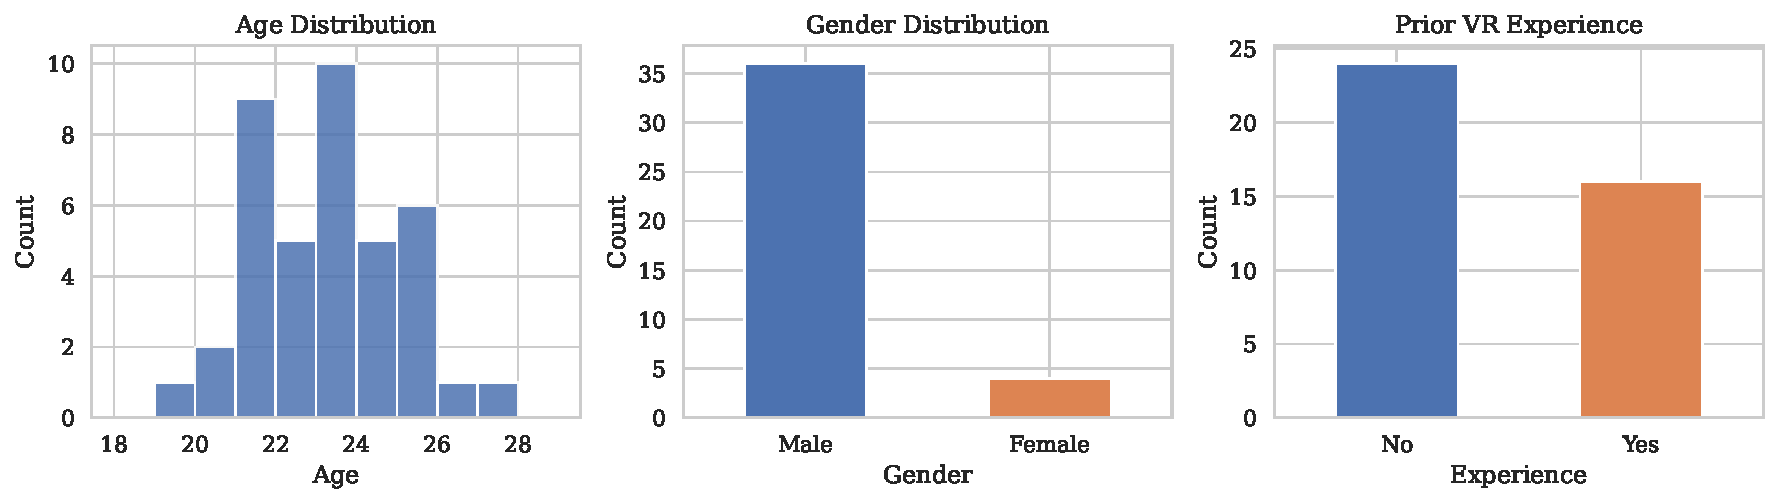
\includegraphics[width=\textwidth]{figures/fig1_demographics.pdf}
    \caption{Distributions of age, gender, and prior VR experience across the 40 participants.}
    \label{fig:demographics}
\end{figure}

\subsection{Clinical Measures}

PHQ-9 scores ranged from 0 to 18 ($M = 6.03$, $SD = 4.63$, $Mdn = 4.5$), with 50\% of participants in the minimal range (0--4), 30\% mild (5--9), 12.5\% moderate (10--14), and 7.5\% moderately severe (15--19). Eight participants (20\%) met the threshold for moderate depression (PHQ-9 $\geq 10$). GAD-7 scores ranged from 0 to 18 ($M = 5.00$, $SD = 4.31$). STAI-T scores ranged from 21 to 73 ($M = 45.00$, $SD = 14.63$).

Shapiro-Wilk tests indicated that both PHQ-9 ($W = 0.897$, $p = .002$) and GAD-7 ($W = 0.883$, $p < .001$) distributions deviated significantly from normality, with a positive skew reflecting the predominantly non-clinical sample. STAI-T was marginally non-normal ($W = 0.944$, $p = .045$).

\begin{figure}[H]
    \centering
    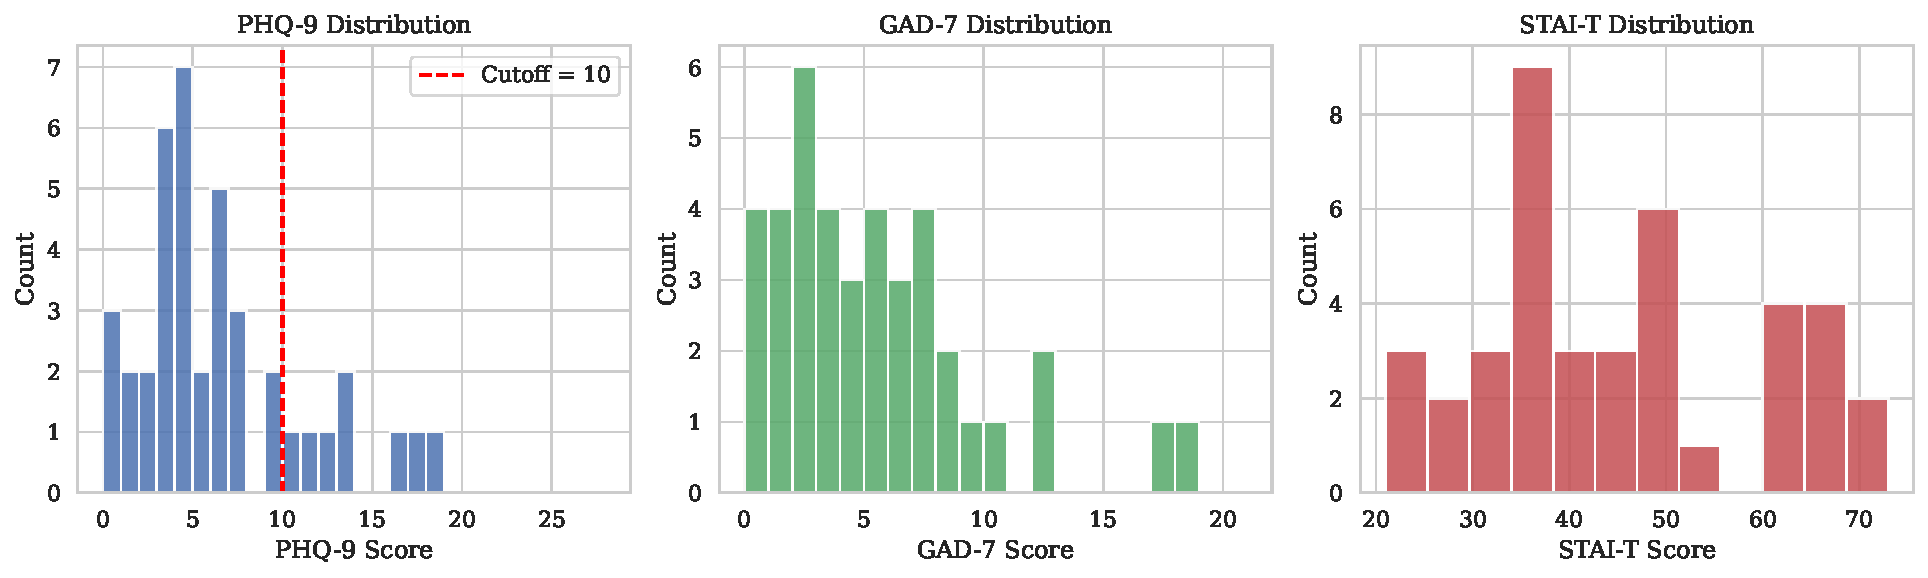
\includegraphics[width=\textwidth]{figures/fig2_clinical_distributions.pdf}
    \caption{Distributions of PHQ-9, GAD-7, and STAI-T scores. The dashed red line on PHQ-9 indicates the clinical cutoff ($\geq 10$) for moderate depression.}
    \label{fig:clinical}
\end{figure}

\begin{figure}[H]
    \centering
    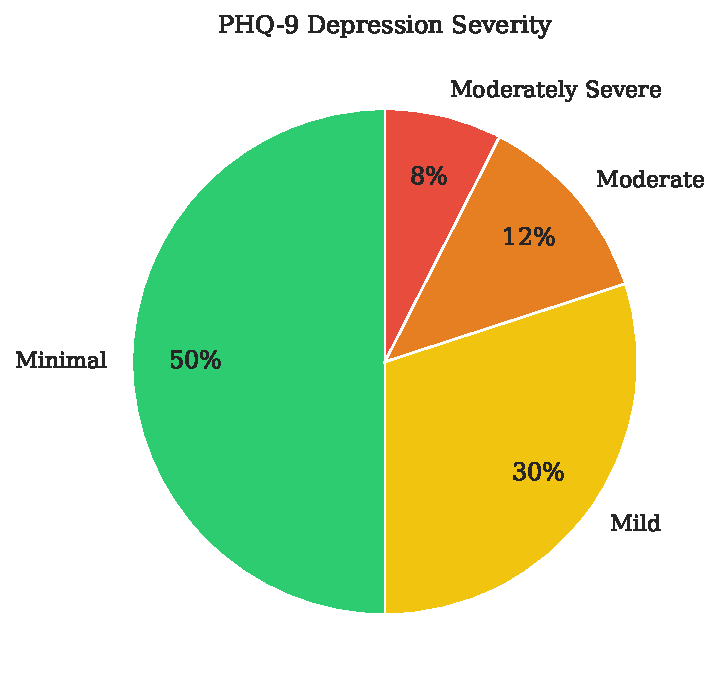
\includegraphics[width=0.45\textwidth]{figures/fig3_phq_severity.pdf}
    \caption{PHQ-9 depression severity classification of participants.}
    \label{fig:severity}
\end{figure}

\subsection{Depression--Anxiety Covariance}

PHQ-9 and GAD-7 were strongly correlated (Pearson $r = .579$, $p < .001$), consistent with the well-documented comorbidity of depression and anxiety \citep{kalin2020anxiety}. PHQ-9 and STAI-T were also strongly correlated ($r = .642$, $p < .001$). These moderate-to-strong correlations underscore the need to control for anxiety when isolating depression-specific effects on headtracking behavior.

\begin{figure}[H]
    \centering
    \begin{subfigure}[b]{0.48\textwidth}
        \centering
        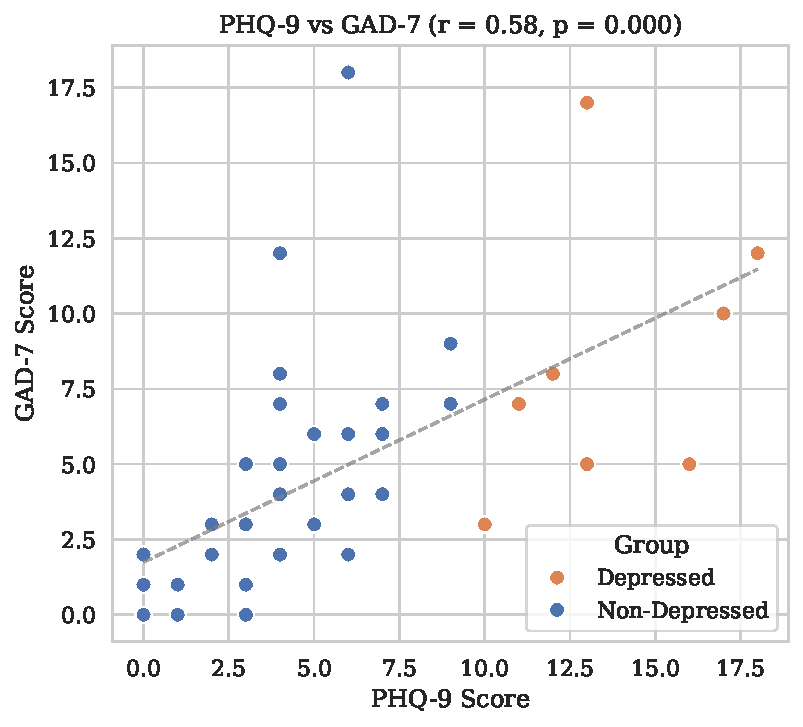
\includegraphics[width=\textwidth]{figures/fig7_phq_vs_gad.pdf}
        \caption{PHQ-9 vs.\ GAD-7 scatter plot.}
    \end{subfigure}
    \hfill
    \begin{subfigure}[b]{0.48\textwidth}
        \centering
        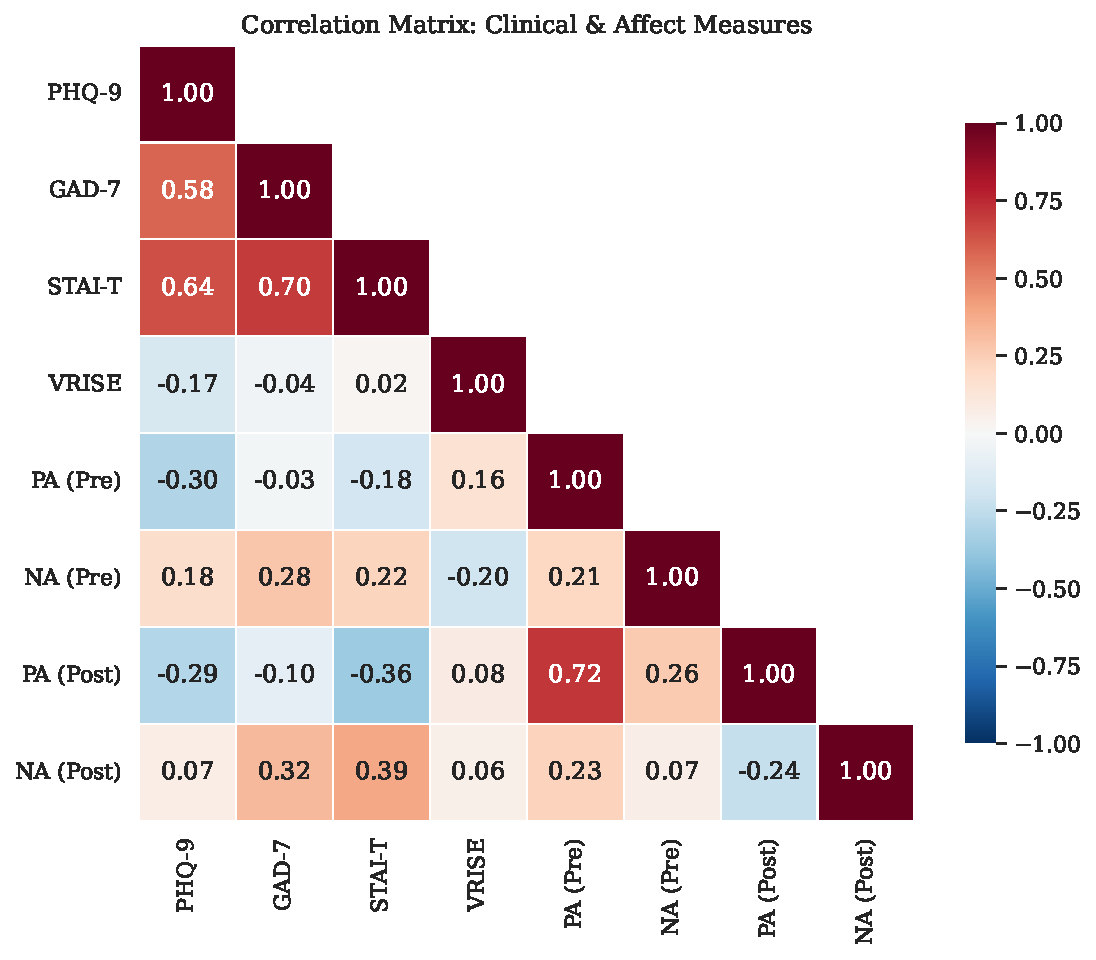
\includegraphics[width=\textwidth]{figures/fig4_correlation_heatmap.pdf}
        \caption{Correlation heatmap of clinical and affect measures.}
    \end{subfigure}
    \caption{(a) Scatterplot showing the strong positive relationship between PHQ-9 and GAD-7 scores. (b) Correlation matrix showing inter-relationships among all clinical and affect measures.}
    \label{fig:correlations}
\end{figure}

\subsection{Video-Level Emotional and Presence Ratings}

The five videos elicited distinct emotional profiles (Table~\ref{tab:video_ratings}). V5 (Tahiti Surf) received the highest valence ($M = 7.12$) and arousal ($M = 6.50$), while V4 (Horror) had the lowest valence ($M = 3.67$) but high arousal ($M = 5.95$). V1 (Abandoned Buildings) scored highest on presence ($M = 29.60$), while V4 scored lowest ($M = 19.85$).

\begin{table}[H]
\centering
\caption{Mean (SD) valence, arousal, and presence scores by video.}
\label{tab:video_ratings}
\begin{tabular}{lccc}
\toprule
\textbf{Video} & \textbf{Valence} & \textbf{Arousal} & \textbf{Presence} \\
\midrule
V1: Abandoned Buildings & 5.20 (1.67) & 4.60 (2.22) & 29.60 (4.41) \\
V2: Beach & 6.53 (1.75) & 4.65 (2.03) & 27.25 (5.31) \\
V3: Campus & 6.15 (1.61) & 4.33 (2.16) & 26.95 (4.52) \\
V4: Horror (Nun) & 3.67 (1.85) & 5.95 (1.68) & 19.85 (5.44) \\
V5: Tahiti Surf & 7.12 (1.68) & 6.50 (1.69) & 28.02 (4.79) \\
\bottomrule
\end{tabular}
\end{table}

\begin{figure}[H]
    \centering
    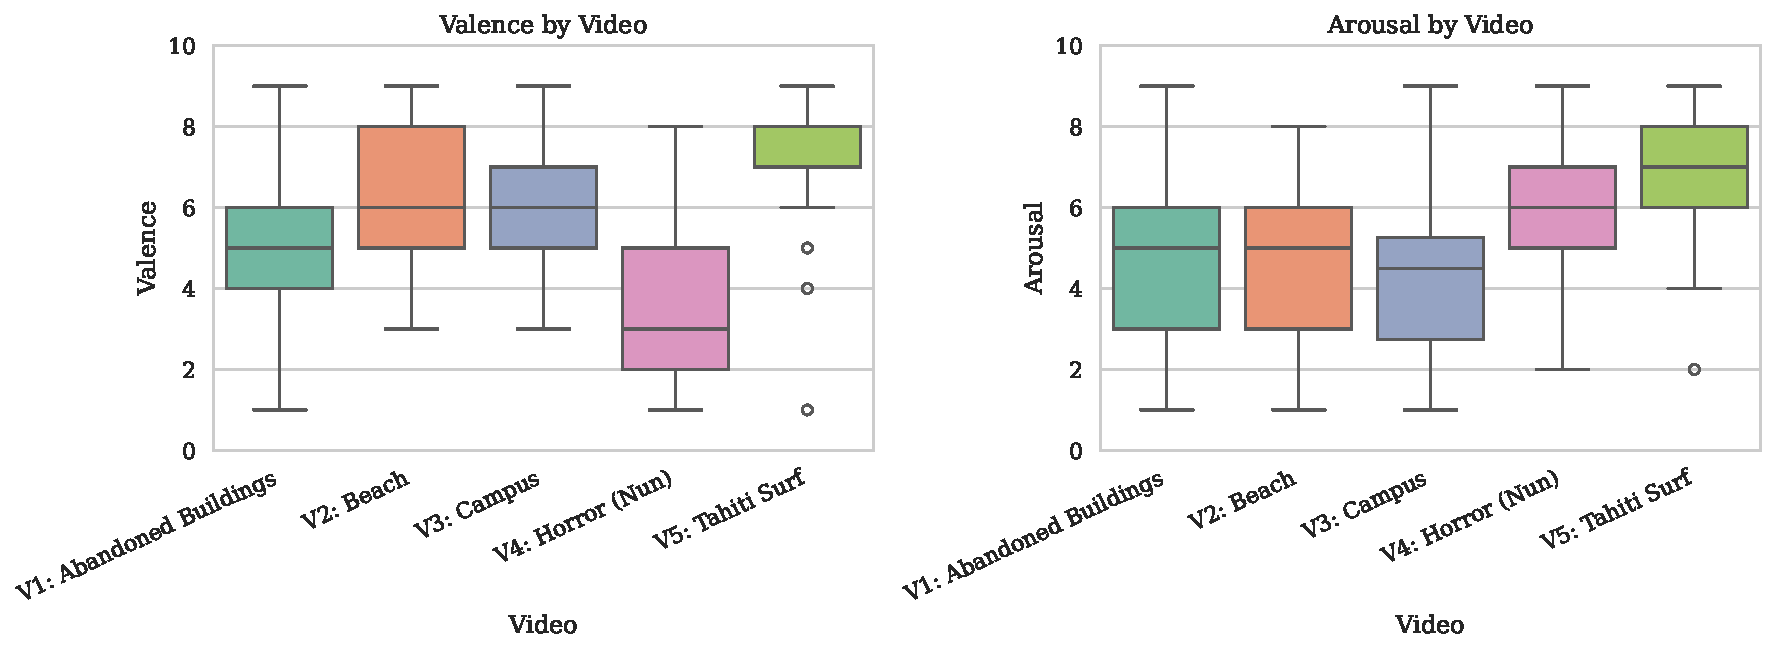
\includegraphics[width=\textwidth]{figures/fig5_valence_arousal_by_video.pdf}
    \caption{Box plots of valence and arousal ratings across the five videos.}
    \label{fig:valence_arousal}
\end{figure}

\begin{figure}[H]
    \centering
    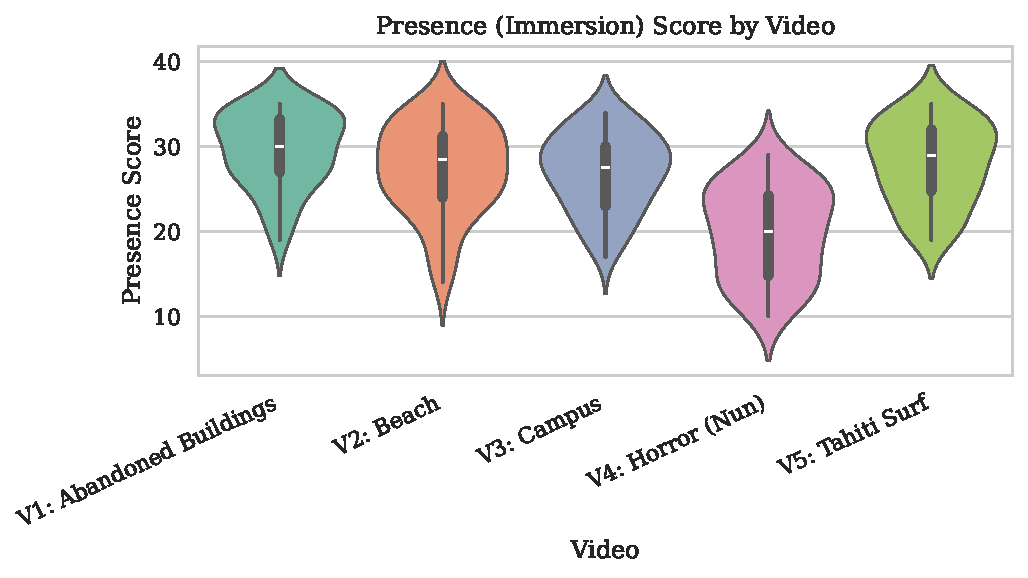
\includegraphics[width=0.65\textwidth]{figures/fig6_presence_by_video.pdf}
    \caption{Violin plots of presence (immersion) scores by video. V4 (Horror) had notably lower presence, possibly due to lower visual quality.}
    \label{fig:presence}
\end{figure}

\subsection{Headtracking Measures}

Descriptive analysis revealed that mean rotation speed varied across videos. V1 (Abandoned Buildings) elicited the highest mean speed ($M = 39.08$°/s), consistent with the exploratory nature of the environment, while V4 (Horror) had the lowest ($M = 24.17$°/s), possibly because the horror narrative directed gaze toward specific focal points. Formal testing of speed differences across videos (one-way ANOVA) is deferred to Report~2.

\begin{figure}[H]
    \centering
    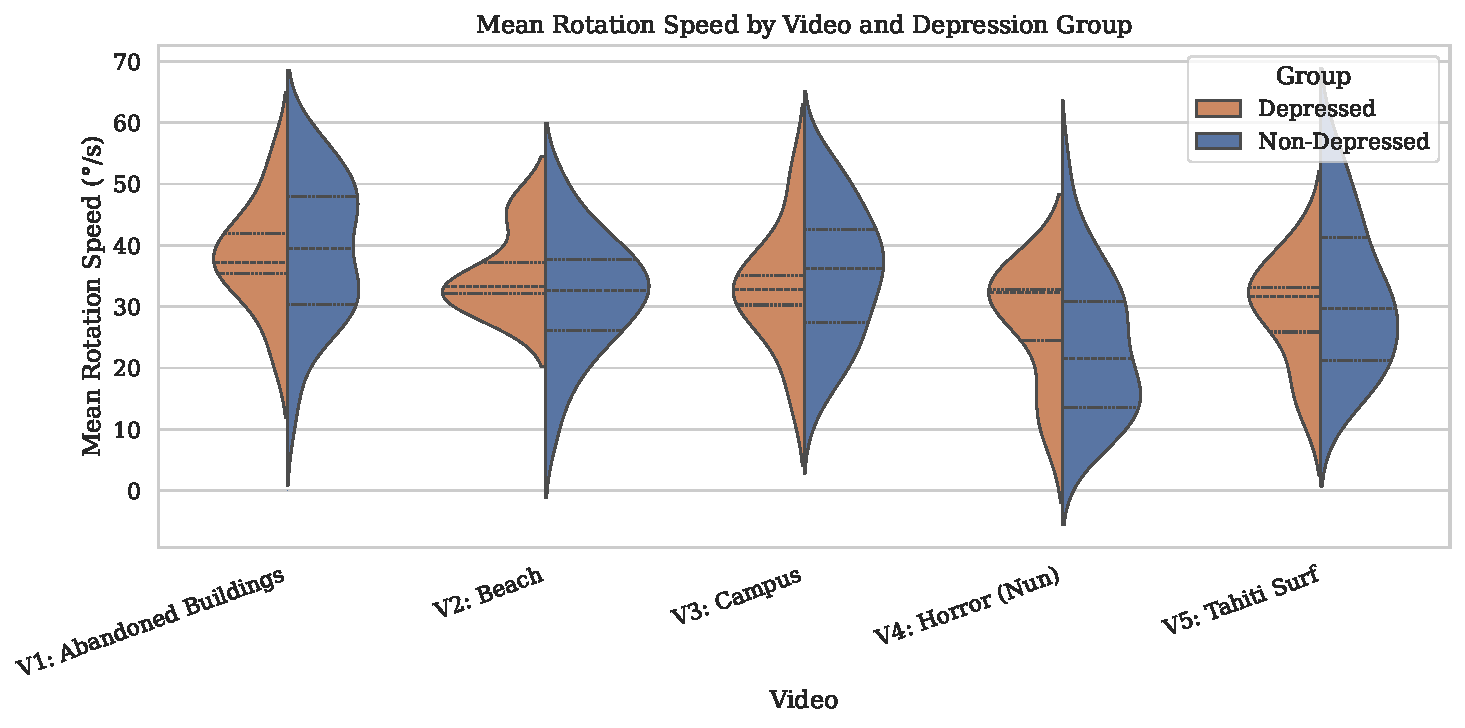
\includegraphics[width=\textwidth]{figures/fig8_headtrack_speed_by_group.pdf}
    \caption{Violin plots of mean rotation speed by video and depression group. Split violins show the distribution for Non-Depressed (blue) and Depressed (orange) groups.}
    \label{fig:speed_violin}
\end{figure}

\subsection{Headtracking by Depression Group}

Welch's independent-samples $t$-tests comparing depressed and non-depressed groups on headtracking measures yielded largely non-significant results (Table~\ref{tab:ttest_results}). At the uncorrected $\alpha = .05$ level, only one of 25 comparisons reached significance: \textbf{V4 (Horror)} total angular range ($t = 2.21$, $p = .048$, Cohen's $d = 0.83$), where the depressed group explored a \textit{greater} angular range. After Bonferroni correction ($\alpha_{\text{corrected}} = .002$ for 25 comparisons), \textbf{no comparisons remained significant}. This finding runs counter to the psychomotor retardation hypothesis and is likely a Type~I error.

Pearson correlations between PHQ-9 scores and participant-averaged headtracking measures were near zero and non-significant: mean total speed ($r = -.060$, $p = .712$), mean yaw speed ($r = -.081$, $p = .617$), and SD of total speed ($r = -.158$, $p = .329$).

\begin{table}[H]
\centering
\caption{Selected Welch's $t$-test results for mean total speed and total angular range by depression group per video. Cohen's $d$ quantifies effect size. No comparison survived Bonferroni correction ($\alpha_{\text{corrected}} = .002$).}
\label{tab:ttest_results}
\small
\begin{tabular}{lcccccc}
\toprule
\textbf{Video} & \multicolumn{3}{c}{\textbf{Mean Speed (Total)}} & \multicolumn{3}{c}{\textbf{Total Angular Range}} \\
\cmidrule(lr){2-4} \cmidrule(lr){5-7}
 & $t$ & $p$ & $d$ & $t$ & $p$ & $d$ \\
\midrule
V1: Abandoned Buildings & $-0.24$ & .816 & $-0.08$ & $-0.22$ & .831 & $-0.07$ \\
V2: Beach & $1.22$ & .239 & $0.38$ & $1.76$ & .104 & $0.65$ \\
V3: Campus & $-0.64$ & .532 & $-0.24$ & $0.16$ & .878 & $0.05$ \\
V4: Horror (Nun) & $1.07$ & .303 & $0.37$ & $2.21$ & .048 & $0.83$ \\
V5: Tahiti Surf & $-0.66$ & .523 & $-0.21$ & $-0.36$ & .727 & $-0.16$ \\
\bottomrule
\end{tabular}
\end{table}

\begin{figure}[H]
    \centering
    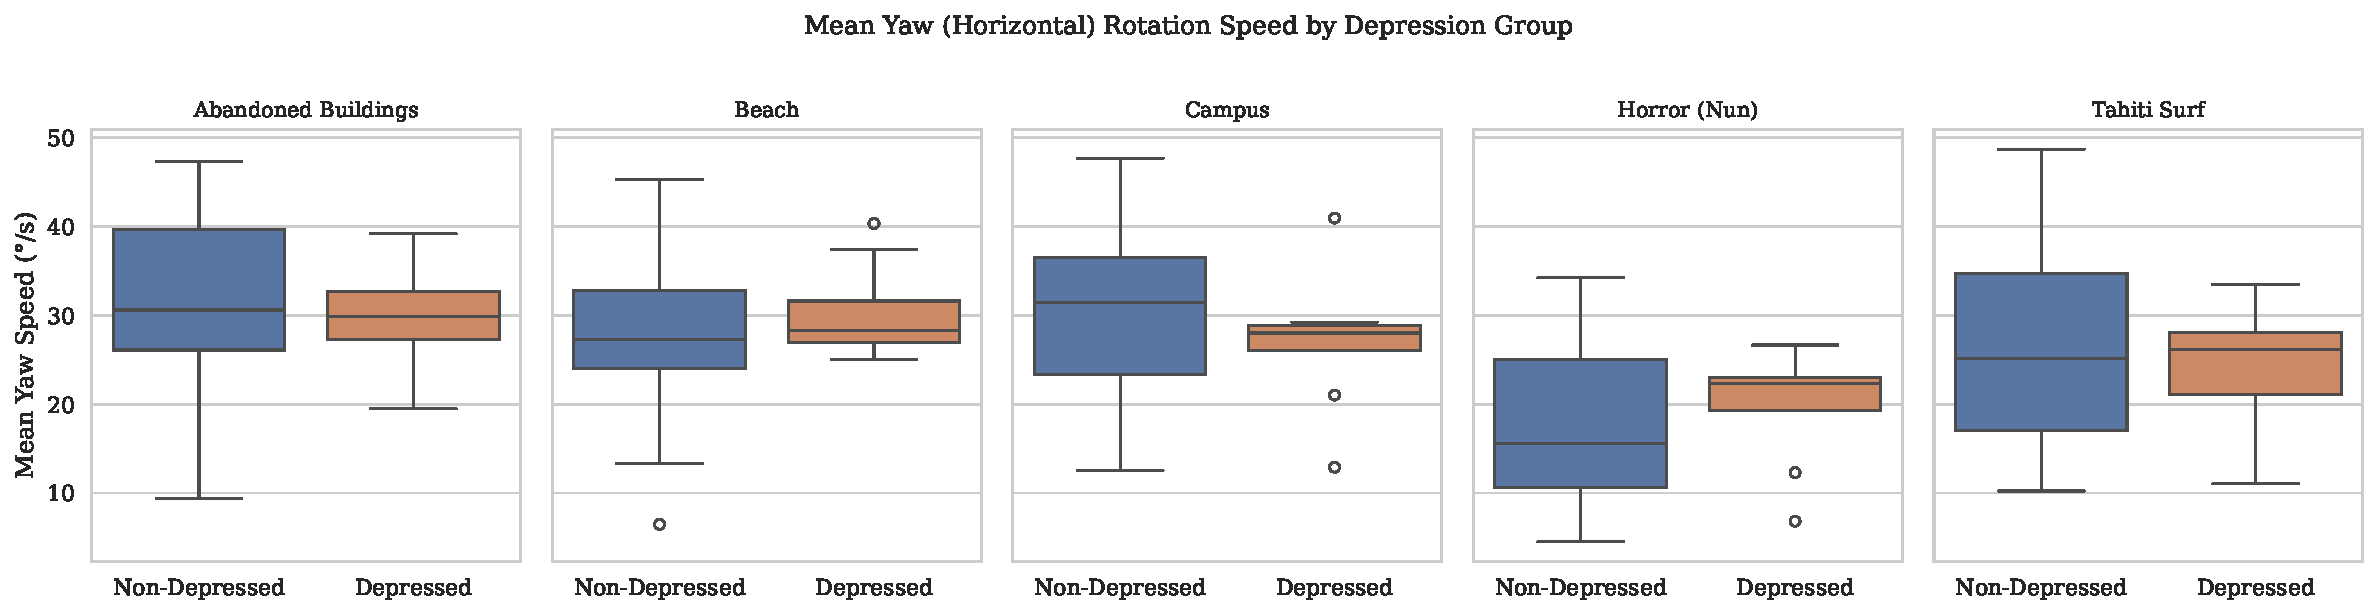
\includegraphics[width=\textwidth]{figures/fig12_yaw_speed_by_group.pdf}
    \caption{Mean yaw (horizontal) rotation speed by depression group for each video.}
    \label{fig:yaw_speed}
\end{figure}

\begin{figure}[H]
    \centering
    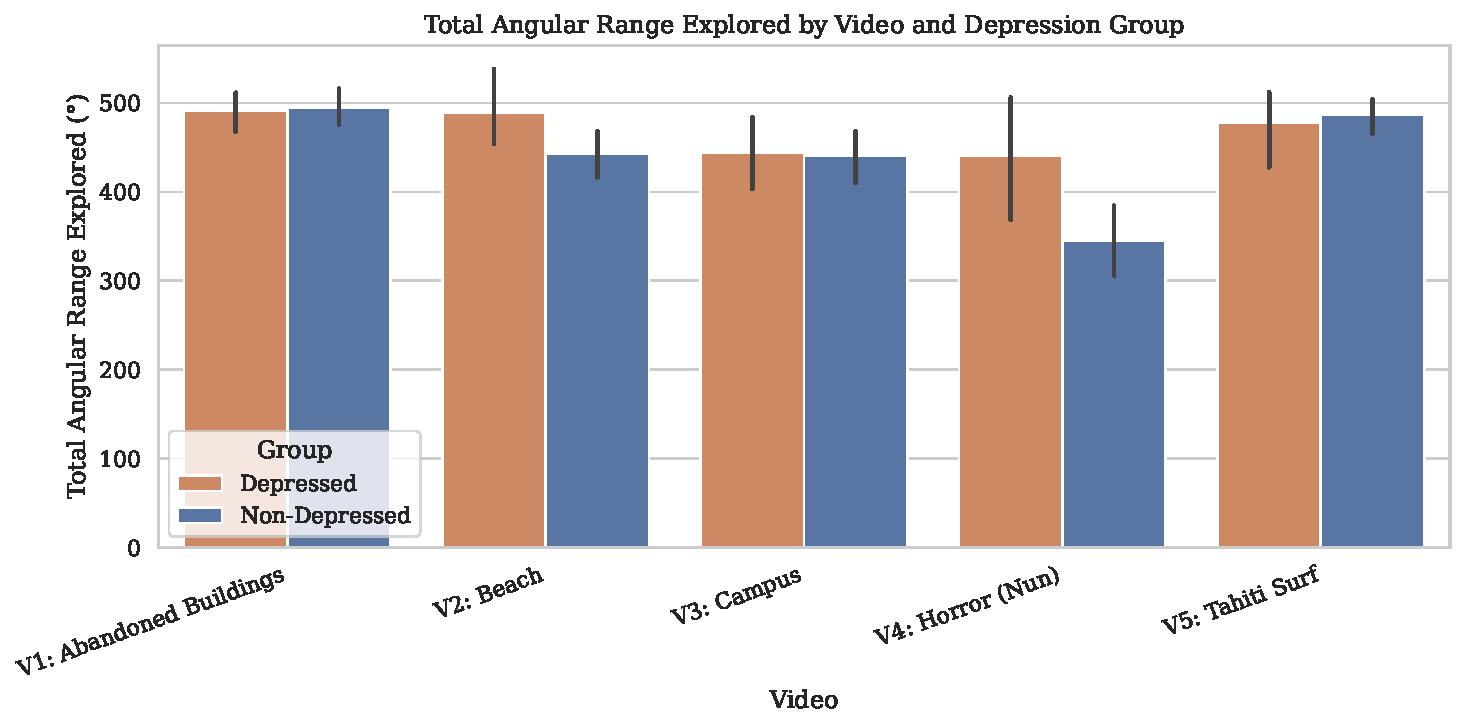
\includegraphics[width=\textwidth]{figures/fig10_angular_range_by_group.pdf}
    \caption{Total angular range explored by video and depression group. Error bars represent 95\% confidence intervals.}
    \label{fig:angular_range}
\end{figure}

\subsection{PANAS: Pre- and Post-VR Mood}

Positive Affect decreased significantly from pre-VR ($M = 34.52$) to post-VR ($M = 32.15$; paired $t(39) = 2.09$, $p = .043$, Cohen's $d = -0.33$). Negative Affect showed a non-significant increase ($M = 12.70 \to 13.95$; $t(39) = -1.06$, $p = .294$, $d = 0.17$).

\begin{figure}[H]
    \centering
    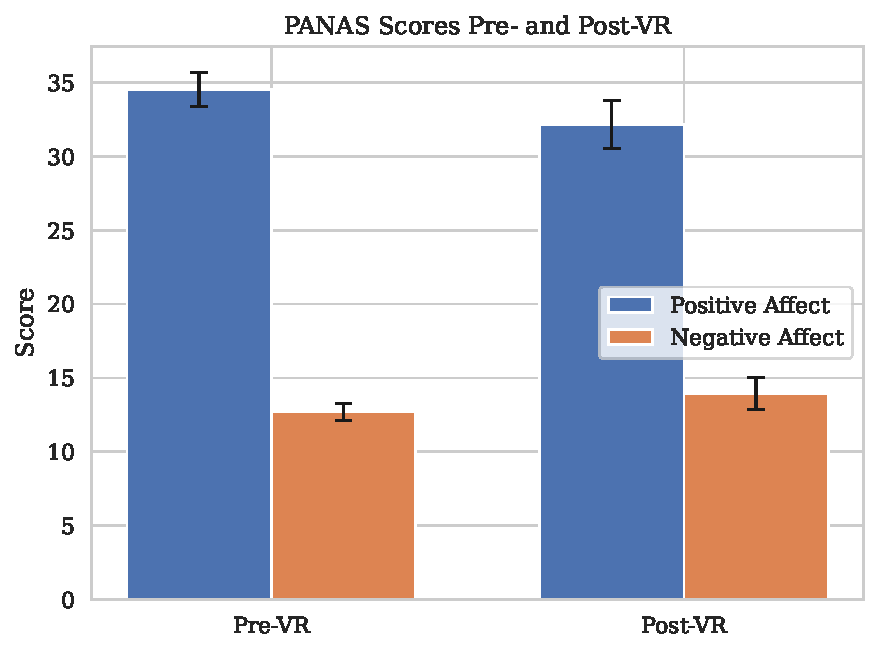
\includegraphics[width=0.55\textwidth]{figures/fig11_panas_change.pdf}
    \caption{PANAS positive and negative affect scores before and after VR exposure. Error bars represent standard errors.}
    \label{fig:panas}
\end{figure}

\subsection{Outlier Analysis}

Using the IQR method, 3 PHQ-9 outliers (scores $> 14.2$) and 2 GAD-7 outliers (scores $> 14.5$) were identified. However, these represent genuine clinical variability (moderately severe depression/anxiety) and were retained. No headtracking speed outliers exceeded $|z| > 3$. One participant had a low VRISE score (17), suggesting possible simulator sickness; this participant was retained but flagged for sensitivity analysis.

% ──────────────────────────────────────────────────────────────────────────────
\section{Conclusion and Future Directions}
% ──────────────────────────────────────────────────────────────────────────────

\subsection{Summary of Findings}
\begin{enumerate}
    \item The sample is predominantly non-clinical: 80\% of participants scored below the moderate depression threshold (PHQ-9 $< 10$), with only 8 in the ``depressed'' group.
    \item Depression and anxiety are strongly correlated (Pearson $r = .58$), confirming the need to account for this covariance in subsequent analyses.
    \item Videos elicited distinct emotional profiles, and descriptive patterns suggest headtracking speed varies across videos (V1 highest at 39.08°/s, V4 lowest at 24.17°/s). Formal one-way ANOVA testing is deferred to Report~2.
    \item Welch's $t$-tests showed \textbf{no significant differences} in mean headtracking speed between depressed and non-depressed groups for any video. After Bonferroni correction for 25 comparisons ($\alpha_{\text{corrected}} = .002$), no comparison reached significance. The original study's finding of significantly reduced scanning speed in the moderate-severe depression group \citep{srivastava2025headscan} was \textbf{not replicated} in this preliminary analysis, likely due to limited statistical power.
    \item One uncorrected-significant effect was found for angular range in V4 (Horror) ($t = 2.21$, $p = .048$, $d = 0.83$), but in the opposite direction to expectations and non-significant after Bonferroni correction---likely a Type~I error.
    \item Positive affect decreased significantly after VR exposure (paired $t$-test: $p = .043$, $d = -0.33$).
\end{enumerate}

\subsection{Limitations}
The key limitation is the small and unbalanced sample ($n_{\text{dep}} = 8$ vs.\ $n_{\text{nondep}} = 32$), which severely limits statistical power. The predominantly male sample (90\%) limits generalizability. Additionally, the current binary classification does not exploit the full range of PHQ-9 scores.

\subsection{Plans for Report 2}
\begin{enumerate}
    \item Use PHQ-9 as a continuous predictor in regression/GLM models, rather than relying solely on categorical grouping, to exploit the full range of scores.
    \item Include GAD-7 and STAI-T as covariates (ANCOVA or multiple regression) to disentangle depression from anxiety effects on headtracking, following the approach of \\citet{srivastava2025headscan}.
    \item Conduct repeated-measures analyses (mixed-effects models or repeated-measures ANOVA) to account for the within-subject structure across 5 videos.
    \item Investigate video-type interactions: do different emotional contexts (positive, negative, neutral, horror) moderate the depression--headtracking relationship?
    \item Perform mediation/moderation analysis with presence and simulator sickness scores.
    \item Conduct effect-size-based power analysis to quantify the statistical power of the current sample and determine what effect sizes are detectable.
    \item Compare results using alternative multiple-comparison corrections (Holm, Benjamini-Hochberg) alongside Bonferroni.
    \item Conduct one-way ANOVA ($F$-test) to formally test whether mean headtracking speed differs significantly across the five videos, with $\eta^2$ as effect size.
\end{enumerate}

% ──────────────────────────────────────────────────────────────────────────────
% References
% ──────────────────────────────────────────────────────────────────────────────
\bibliographystyle{apalike}

\begin{thebibliography}{99}

\bibitem[Srivastava et al., 2025]{srivastava2025headscan}
Srivastava, P., Lahane, R., Vivek, R., \& Pulapa, P. (2025).
What Do Head Scans Reveal About Depression? Insights from 360° Psychomotor Assessment.
\textit{Proceedings of the Annual Meeting of the Cognitive Science Society}, 47(0).
\url{https://escholarship.org/uc/item/8n15r08z}

\bibitem[Bennabi et al., 2013]{bennabi2013psychomotor}
Bennabi, D., Vandel, P., Papaxanthis, C., Pozzo, T., \& Haffen, E. (2013).
Psychomotor retardation in depression: A systematic review of diagnostic, pathophysiologic, and therapeutic implications.
\textit{BioMed Research International}, 2013.

\bibitem[Kalin, 2020]{kalin2020anxiety}
Kalin, N.~H. (2020).
The Critical Relationship Between Anxiety and Depression.
\textit{American Journal of Psychiatry}, 177(5), 365--367.

\bibitem[Kourtesis et al., 2019]{kourtesis2019vrnq}
Kourtesis, P., Collina, S., Doumas, L.~A., \& MacPherson, S.~E. (2019).
Validation of the Virtual Reality Neuroscience Questionnaire.
\textit{Frontiers in Human Neuroscience}, 13, 417.

\bibitem[Kroenke et al., 2001]{kroenke2001phq9}
Kroenke, K., Spitzer, R.~L., \& Williams, J.~B. (2001).
The PHQ-9: Validity of a brief depression severity measure.
\textit{Journal of General Internal Medicine}, 16(9), 606--613.

\bibitem[Russell, 1980]{russell1980circumplex}
Russell, J.~A. (1980).
A circumplex model of affect.
\textit{Journal of Personality and Social Psychology}, 39(6), 1161--1178.

\bibitem[Spielberger et al., 1983]{spielberger1983stai}
Spielberger, C.~D., Gorsuch, R.~L., Lushene, R., Vagg, P.~R., \& Jacobs, G.~A. (1983).
\textit{Manual for the State-Trait Anxiety Inventory}. Consulting Psychologists Press.

\bibitem[Spitzer et al., 2006]{spitzer2006gad7}
Spitzer, R.~L., Kroenke, K., Williams, J.~B., \& L\"{o}we, B. (2006).
A brief measure for assessing generalized anxiety disorder: The GAD-7.
\textit{Archives of Internal Medicine}, 166(10), 1092--1097.

\bibitem[Watson et al., 1988]{watson1988panas}
Watson, D., Clark, L.~A., \& Tellegen, A. (1988).
Development and validation of brief measures of positive and negative affect: The PANAS scales.
\textit{Journal of Personality and Social Psychology}, 54(6), 1063--1070.

\end{thebibliography}

\end{document}
